\documentclass[12pt]{article}

\usepackage[utf8]{inputenc}
\usepackage{mathptmx}
\usepackage{babel}
\usepackage{indentfirst}
\usepackage{ragged2e}
\usepackage{graphicx}
\usepackage{url}
\usepackage{float}
\usepackage{subcaption}
\usepackage[ampersand]{easylist}
\usepackage{gensymb}
\usepackage[12pt]{moresize}
\usepackage{wrapfig}
\usepackage{parskip}
\usepackage{geometry}

\begin{document}
	
	\begin{titlepage} 
		\raggedleft % Baca u desno
		
		\rule{1pt}{\textheight} % VertikQalna linija
		\hspace{0.05\textwidth} % prvi whitespace
		\parbox[b]{0.9\textwidth}{ % box koji drzi desno
			{\Huge\Huge\bfseries SpaceRTS}\\[1\baselineskip] % Naslov
			\vspace{0.35\textheight}
			\parbox[b]{0.9\textwidth}{
				%{\Huge\itshape{Dobre i loše strane}}\\[10\baselineskip] % Podnaslov  % drugi whitespace
			}
			\\[10\baselineskip]
			{\Large\textbf{Patrik Dereh i Josip Šime Zrilić}}\\
			{\Large\textit{1.5, Gimnazija Andrije Mohorovičića Rijeka}}\\
			{\Large{Profesor: Goran Boneta}}\\
			{\Large\textit{08.05.2020}}
		}
	\end{titlepage}
	
	\renewcommand{\contentsname}{Sadržaj}
	\renewcommand{\listfigurename}{\section{Priložene slike}}
	\renewcommand{\figurename}{\scriptsize{Slika}}
	
	\tableofcontents
	
	\newpage
	\section{Uvod}
	
	\subsection{RTS igre}
	Strateške igrice u stvarnom vremenu(RTS) su relativno popularan žanr igrica u kojem jedan ili više igrača gradi carstvo I vojsku kako bi pobjedio protivnika bio taj protivnik drugi igrač ili umjetna inteligencija, ali kako RTS igre moraju imati relativno jednostavan dizajn kako nebi bile zamorne ,a mi smo ljubitelji igrica sa kompleksnijim igračim mehanikama mi smo odlučili kombinirati elemente RTS igrica sa elementima igrica 4X žanra koje generalno imaju kompleksnije mehanike.
	
	\subsection{Ideja}
	Ideju smo smislili jednog ponedjeljka za vrijeme sata povijesti kada smo krenuli malo “razbacivati” ideje. Cilj igrice je preuzeti vlast nad galaksijom ekspanzijom carstva te planetskim I svemiriskim bitkama, Igrač može igrati kao bilo koje od četiri glavna carstva od kojih svako ima svoje posebne mehanike I specijalizaciju. Zhui imaju unaprijed izgrađenu bazu te se primarno bave trgovinom, Scavangeri nemaju snažne razvijene baze niti mogu istraživati nove tehnologije, ali zato mogu sklapati tehnologije drugih carstava jedne s drugima kao I pronalaziti neke davno izgubljene tehnologije , MSEA je carstvo robota koji svoju poplaciju moraju proizvoditi te oni nemaju potrebu za hranom, Ngubu su carstvo cija posebnost lezi u manipulaciji gena, oni mogu svoju populacije genetski manipulirati kako bi se usavršili, a dostupna su im I moćna bio-oružja.
	
	\subsection{O Autorima}
	Mi smo učenici 4.5 razreda Gimnazije Andrije Mohorovičića I odlučili smo napraviti kompleksnu igricu jer je želimo jednog dana monetarizirati na Steam platformi.
	
	\subsection{Izrada projekta}
	Izrada projekta je započela 8.3.2020.
	Za programski jezik smo odabrali C\# zbog njegove brzine I jednostavnosti objektno orijentiranog programiranja u njemu zbog njegova “multiplatmorfiteta”.
	Ovaj projekt predstavlja znatan izazov zbog njegove kompleksnosti stoga je još uvijek u razvoju.
	
	
		\clearpage
	\section{Detaljan opis rada}
	
	\subsection{Main Menu}
		Sadrži opcije:
	\begin{itemize}
		\item	“play” - pokreće testnu verziju igrice
		\item	“exit”- gasi program
		\item	“settings”- ništa jer postavke nisu još dostupne
	\end{itemize}


	\begin{wrapfigure}{R}{1\textwidth}
		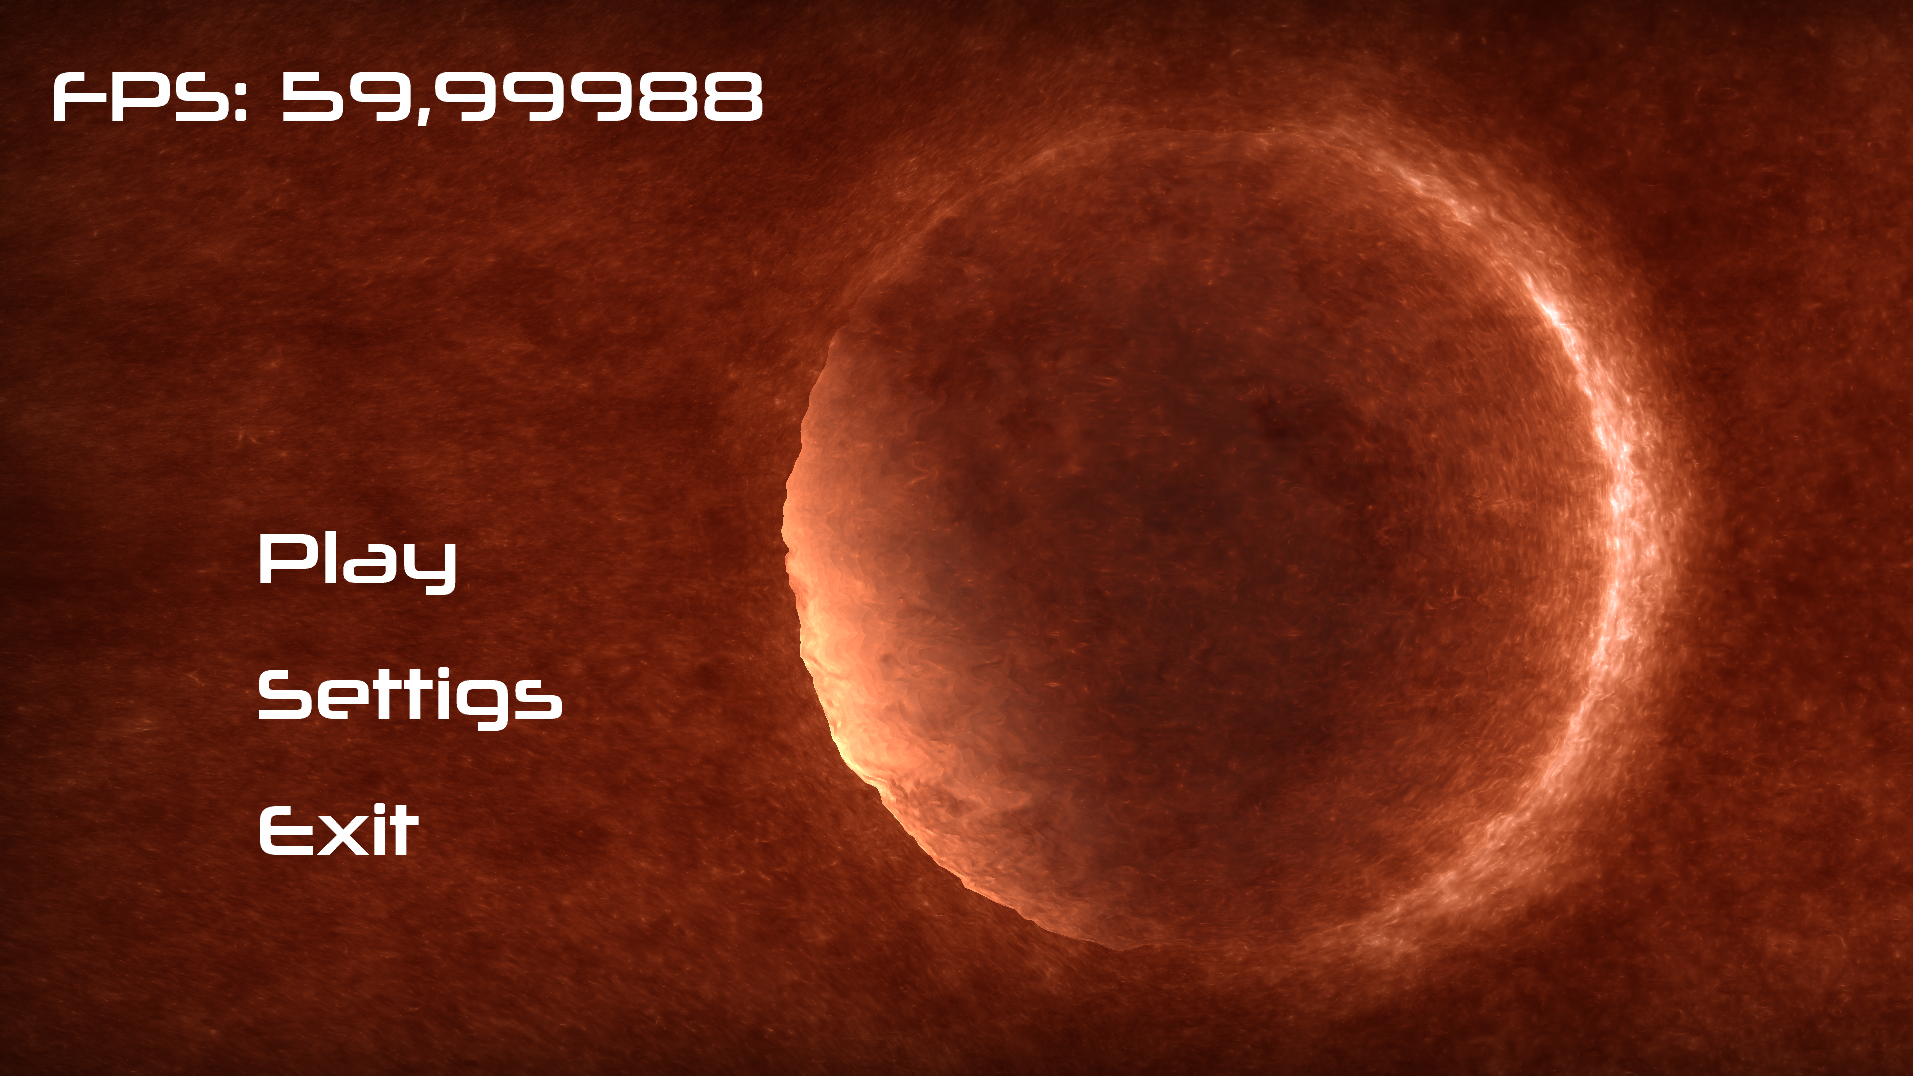
\includegraphics[width=\linewidth]{figures/Slika4.png}
		\caption{Main Menu}
		\label{fig:fig_4}
	\end{wrapfigure}

	
	
	\clearpage
	\subsection{Mapa}
	Teren se generira uz pomoć Perlinovog šuma, algoritma koji generira nasumične vrijednosti koje zajedno imaju prirodnog smisla tj. vrijednosti nisu u potpunosti nasumične nego svaka vrijednost djelomično ovisi o susjednim vrijednostima. Teren je izgrađen od mreže šesterokutnih čelija. Različiti planeti imaju različitu učestalost I amplitudu visinskih promjena kao I različitu učestalost planina, veličine planina I  biome. Nasumično se generiraju izvori rude koji se razlikuju po rijetkosti- zeleni(najčešći),plavi(srednje čest),crveni(najrijeđi). Klikom na teren igrač može postaviti testnu građevinu. 
	
	\begin{wrapfigure}{R}{1\textwidth}
		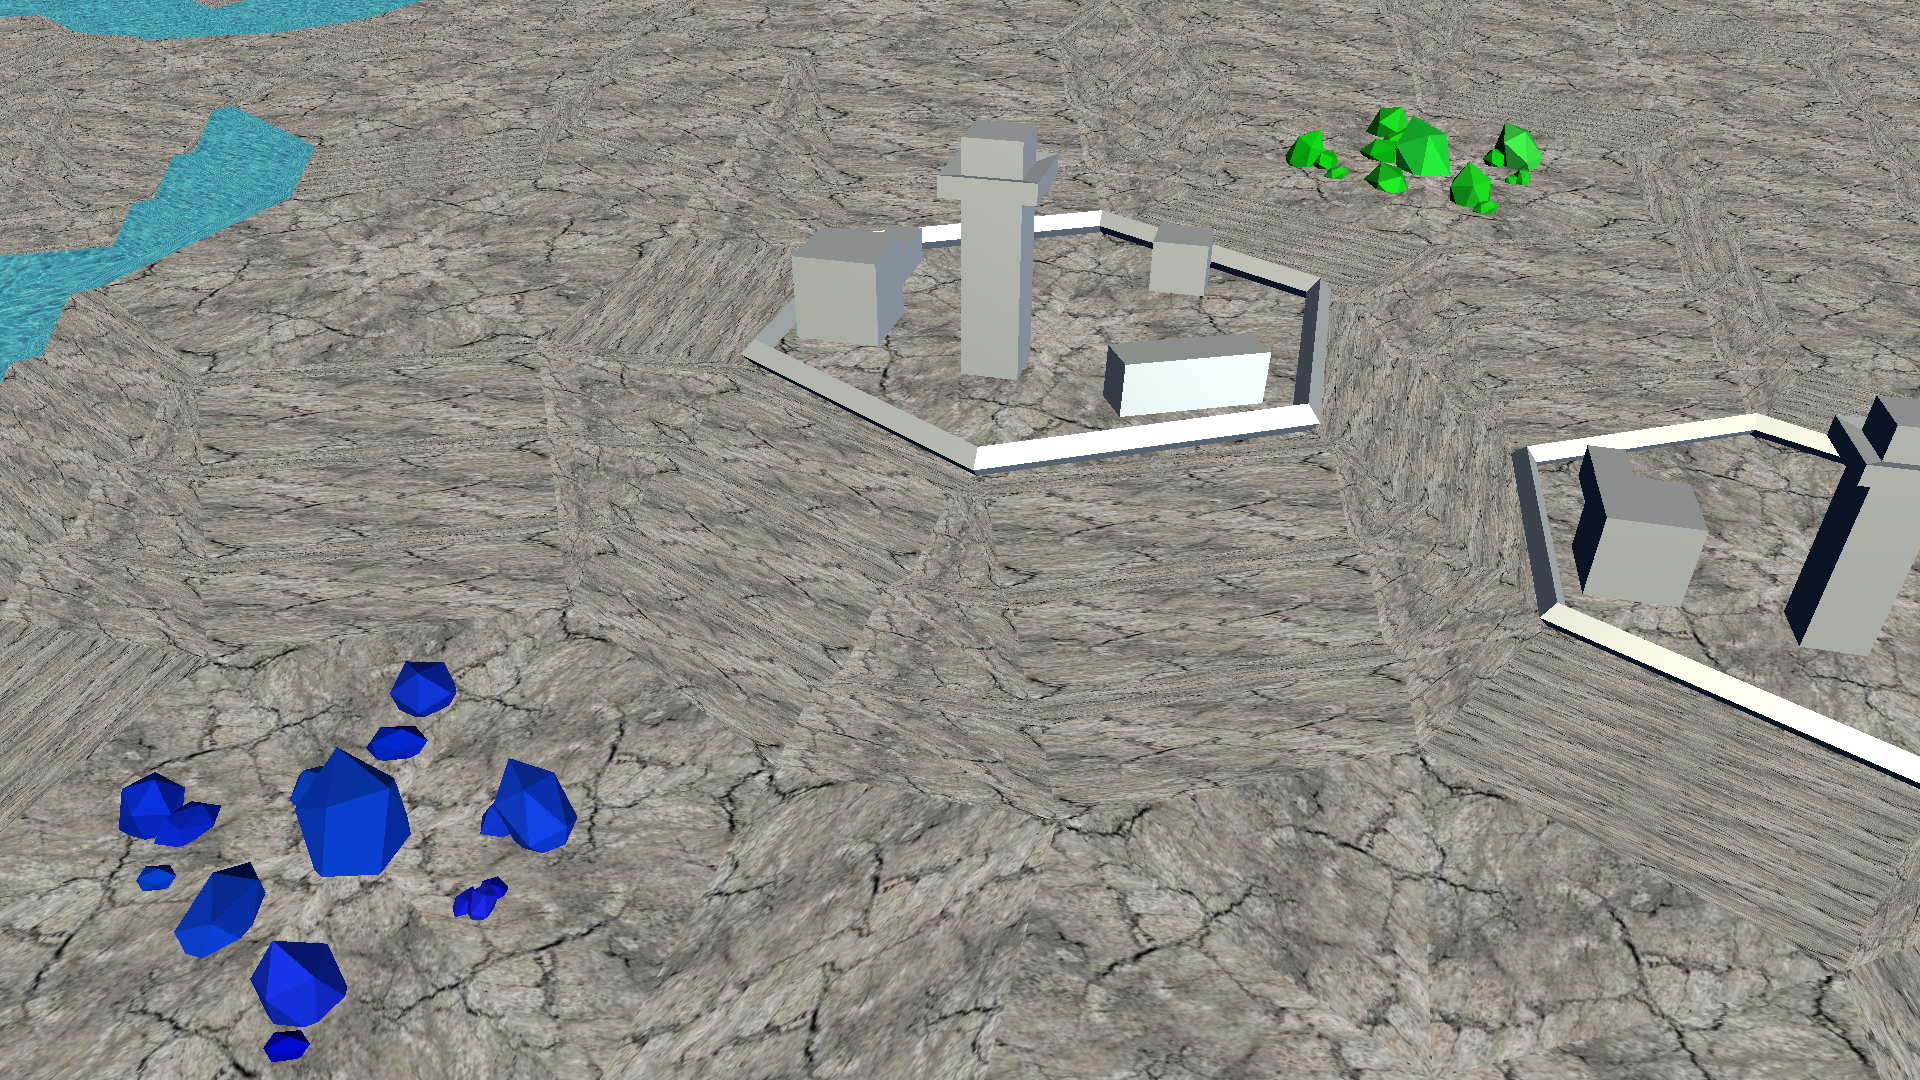
\includegraphics[width=\linewidth]{figures/Slika5.png}
		\caption{Mapa, zelena i plava ora, te postavljene testne strukture}
		\label{fig:fig_5}
	\end{wrapfigure}

	\clearpage
	\subsection{Kontrole}
	\begin{itemize}
		\item	WASD tipke kontroliraju kameru
		\item	Esc terminira program
		\item	Lijevi klik postavlja građevinu u čeliju
	\end{itemize}
	
	\clearpage
	\section{Tehničke informacije}
	\subsection{Sistemska konfiguracija}
	Igra je iznimno optimizirana, te ne zahtjeva jako računalo za pokrenuti
	
	\subsubsection{Minimalna sistemska konfiguracija}
	\begin{itemize}
		\item	Ryzen 3 1200
		\item	4GB RAM-a
		\item	Nvidia GTX 820M
		\item	256MB slobodnog prostora
		\item 	os: bilo koji 32 ili 64 bitni
	\end{itemize}
	
	\subsubsection{Testirana sistemska konfiguracija}
	\begin{itemize}
		\item	Intel Core i5-9300H
		\item	16GB RAM-a
		\item	Nvidia GTX 1660 Ti
		\item	256MB slobodnog prostora
		\item 	os: Arch Linux
	\end{itemize}

	\subsubsection{Preopručena sistemska konfiguracija}
	\begin{itemize}
		\item	Intel Core i5-9300H
		\item	16GB RAM-a
		\item	Nvidia GTX 1660 Ti
		\item	256MB slobodnog prostora
		\item 	os: Arch Linux
	\end{itemize}	
	
	\clearpage
	\subsection{Korištene tehnologije}
	Korištene tehnologije su brze, sigurne i pouzdane, te je većina njih otvorena koda.
	\begin{itemize}
		\item	Visual studio code
		\item	Monodevelop
		\item	C\#
		\item	Mono
		\item	HLSL, DirectX
		\item	Monogame
		\item	Blender
	\end{itemize}

	\begin{wrapfigure}{R}{1\textwidth}
		\includegraphics[width=\linewidth]{figures/Slika6.png}
		\caption{Korištene tehnologije}
		\label{fig:fig_5}
	\end{wrapfigure}
	
	\clearpage
	\section{Održivost}
	
	\subsection{Planovi za budućnost}
	U narednim mjesecima igra će dalje napredovati, te bi do kraja ljeta trebala biti u potpunosti gotova.
	
	\subsection{Dokumentacija koda}
	Kod je dobro dokumentiran - zbog korištenja tehnologije doxygen, te je iznimno samo-objašnjiv, pružajući nam mogućnosti lagnih i brzih unapređenja i popravaka.
	\clearpage		
	
	\newpage	
	\begin{appendix}
		\listoffigures
	\end{appendix}
	
\end{document}
